\documentclass{article}
\usepackage[utf8]{inputenc}
\usepackage[margin=2cm]{geometry}
\usepackage{fullpage,enumitem,amssymb,amsmath,xcolor,cancel,gensymb,hyperref,graphicx}
\usepackage{indentfirst}
\usepackage{multirow}
\usepackage{booktabs}
\setlength{\parskip}{1em}
\usepackage{subfig}
\usepackage[framed,numbered,autolinebreaks,useliterate]{mcode}
\usepackage{url,textcomp}
\usepackage{graphicx}
\usepackage{float}
\graphicspath{{Figures/}{logo/}} 
%\begin{align*}…\end{align*} if you want to fit an equation. 
%FOR PICTURES: include graphicsx 
%\includegraphics[scale=x]{name}
%double space and write caption in the center classshe 

\title{MTH208 Coursework (S2, AY2020-21) \\ Buckling of a Circular Ring}
\author{Ziniu Wu (1824944)}
\date{May 25th, 2021}


\begin{document}
	
\maketitle

\section*{Problem Formation} 
A system of seven differential equations serves as a model for a circular ring with compressibility c, under hydrostatic pressure p coming from all directions. The model will be nondimensionalized for simplicity, and we will assume that the ring has radius 1 with horizontal and vertical symmetry in the absence of external pressure.

The model accounts for only the upper left quarter of the ring—the rest can be filled
in by the symmetry assumption. The independent variable s represents arc length along the
original centerline of the ring, which goes from $s = 0$ to $s = \frac{\pi}{2}$. The dependent variables
at the point specified by arc length s are as follows:

$$
\begin{array}{l}
	y_{1}(s)=\text { angle of centerline with respect to horizonta } \\ 
	y_{2}(s)=x \text { -coordinate } \\ 
	y_{3}(s)=y \text { -coordinate } \\ 
	y_{4}(s)=\text { arc length along deformed centerline } \\ 
	y_{5}(s)=\text { internal axial force } \\ 
	y_{6}(s)=\text { internal normal force } \\ 
	y_{7}(s)=\text { bending moment. }
\end{array}
$$

The boundary value problem formed as Huddleston [2000]:

$$
\begin{array}{l}
	y_{1}^{\prime}=-1-c y_{5}+(c+1) y_{7} \\
	y_{2}^{\prime}=\left(1+c\left(y_{5}-y_{7}\right)\right) \cos y_{1} \\
	y_{3}^{\prime}=\left(1+c\left(y_{5}-y_{7}\right)\right) \sin y_{1} \\
	y_{4}^{\prime}=1+c\left(y_{5}-y_{7}\right) \\
	y_{5}^{\prime}=-y_{6}\left(-1-c y_{5}+(c+1) y_{7}\right) \\
	y_{6}^{\prime}=y_{7} y_{5}-\left(1+c\left(y_{5}-y_{7}\right)\right)\left(y_{5}+p\right) \\
	y_{7}^{\prime}=\left(1+c\left(y_{5}-y_{7}\right)\right) y_{6}
\end{array}
$$

where
$y_{1}(0)=\frac{\pi}{2}$, $y_{1}(\frac{\pi}{2})=0$,
$y_{2}(\frac{\pi}{2})=0$,
$y_{3}(0)=0$,
$y_{4}(0)=0$,
$y_{6}(0)=0$,
$y_{6}(\frac{\pi}{2})=0$.

The following circular solution (7.10) to the boundary value problem exists for any choice of parameters c and p:

$$
\begin{array}{l}
	y_{1}(s)=\frac{\pi}{2}-s\\ 
	y_{2}(s)=\frac{c+1}{c p+c+1}(-\cos s)\\ 
	y_{3}(s)=\frac{c+1}{c p+c+1} \sin s\\ 
	y_{4}(s)=\frac{c+1}{c p+c+1} s\\ 
	y_{5}(s)=-\frac{c+1}{c p+c+1} p\\ 
	y_{6}(s)=0\\ 
	y_{7}(s)=-\frac{c p}{c p+c+1}
\end{array}
$$

The critical pressure depends on the compressibility of the ring. The smaller the parameter
c, the less compressible the ring is, and the lower the critical pressure at which it changes
shape instead of compressing in original shape. 

\section*{Question 1} 
Verify that (7.10) is a solution of the BVP for each compressibility c and pressure p.

\textbf{Solution:} 

In order to verify that (7.10) is a solution of the BVP for each compressibility c and pressure p. We need to find the first order derivative  with repect to s of (7.10):

$$
\begin{array}{l}
	y^{'}_{1}(s)=-1\\ 
	y^{'}_{2}(s)=\frac{c+1}{c p+c+1}\sin s\\ 
	y^{'}_{3}(s)=\frac{c+1}{c p+c+1} \cos s\\ 
	y^{'}_{4}(s)=\frac{c+1}{c p+c+1}\\ 
	y^{'}_{5}(s)=0\\ 
	y^{'}_{6}(s)=0\\ 
	y^{'}_{7}(s)=0
\end{array}
$$

Then:

$$
\begin{array}{l}
	-1-c y_{5}+(c+1) y_{7} := -1 = y^{'}_{1}(s)\\
	\left(1+c\left(y_{5}-y_{7}\right)\right) \cos y_{1} := (1+ c \frac{-p}{cp+c+1})cos(\frac{\pi}{2}-s) = \frac{c+1}{c p+c+1}\sin s = y^{'}_{2}(s)\\
	\left(1+c\left(y_{5}-y_{7}\right)\right) \sin y_{1}  := (1+ c \frac{-p}{cp+c+1})sin(\frac{\pi}{2}-s) = \frac{c+1}{c p+c+1} \cos s = y^{'}_{3}(s)\\
	1+c\left(y_{5}-y_{7}\right) :=  1+ c \frac{-p}{cp+c+1} = \frac{c+1}{c p+c+1} =  y^{'}_{4}(s)\\
	-y_{6}\left(-1-c y_{5}+(c+1) y_{7}\right) := 0 = y^{'}_{5}(s)\\
	y_{7} y_{5}-\left(1+c\left(y_{5}-y_{7}\right)\right)\left(y_{5}+p\right) := -\frac{c p}{c p+c+1} (-\frac{c+1}{c p+c+1} p)-(-\frac{c+1}{c p+c+1}) (-\frac{c p}{c p+c+1}) = y^{'}_{6}(s)\\
	\left(1+c\left(y_{5}-y_{7}\right)\right) y_{6} := 0 = y^{'}_{7}(s)
\end{array}
$$

satifying the systems of differential equations in the BVP. Then, check the boundary value conditions by taking $s=0$ and $s=\frac{\pi}{2}$ into (7.10):

$y_{1}(0)=\frac{\pi}{2}$, $y_{1}(\frac{\pi}{2})=0$,
$y_{2}(\frac{\pi}{2})=0$,
$y_{3}(0)=0$,
$y_{4}(0)=0$,
$y_{6}(0)=0$,
$y_{6}(\frac{\pi}{2})=0$. 

Hence, (7.10) is a solution of the BVP for each compressibility c and pressure p.


%--------------------------------------------------
%--------------------------------------------------

%--------------------------------------------------
%--------------------------------------------------
\section*{Question 2} 

Set compressibility to the moderate value c = 0.01. Solve the BVP by the \textbf{Shooting Method}
for pressures p = 0 and 3. The function F in the Shooting Method should use the three
missing initial values (y2(0),y5(0),y7(0)) as input and the three final values
(y1($\pi$/2),y2($\pi$/2),y6($\pi$/2)) as output. The multivariate solver \textbf{Broyden II} from Chapter 2 can be used to solve for the roots of F. Compare with the correct solution (7.10). Note that,
for both values of p, various initial conditions for Broyden’s Method all result in the same
solution trajectory. How much does the radius decrease when p increases from 0 to 3?

%--------------------------------------------------
%--------------------------------------------------


\textbf{Solution:} 

Define  $$
\mathbf{s}=\left[\begin{array}{l}
	y_{2}(0) \\
	y_{5}(0) \\
	y_{7}(0)
\end{array}\right]=\left[\begin{array}{l}
s_2 \\
s_5 \\
s_7
\end{array}\right], \mathbf{F}(\mathbf{s})=\left[\begin{array}{l}
	y_{1}\left(\frac{\pi}{2} ; \mathbf{s}\right) \\
	y_{2}\left(\frac{\pi}{2} ; \mathbf{s}\right) \\
	y_{6}\left(\frac{\pi}{2} ; \mathbf{s}\right)
\end{array}\right]
$$ with $\mathbf{y}=(t;s)$ solving the ODEs using ode45 and $$
\mathbf{y}(0 ; s)=\left[\begin{array}{c}
	\frac{\pi}{2} \\
	s_{2} \\
	0 \\
	0 \\
	s_{5} \\
	0 \\
	s_{7}
\end{array}\right]
$$



Then, apply shooting method and broyden method. Therefore, we can solve the problem by the script \textbf{solveQ2.m}:

\begin{lstlisting}
clc;
clear;
%% Q2 and Q3
global c p;
c = 0.01;
p = 3; % Change the value of p here

%% Init
s=[0 0 0 0 0 0 0]; 
s0 = [3;1;0];
sspan = [0 pi/2];
y0 = [pi/2 s(2) 0 0 s(5) 0 s(7)];
yb = [0 0 0 0 0 0 0]; %Value to be Shot
k=100;

%% Solver
% z=F(s0, c, p);

sstar = broyden2(@(s)F(s, c, p), s0, k); 

if (norm(F(sstar, c, p)) < 1e-5)
	disp("sstar found")
	% Plot the Result
	y0 = [pi/2 sstar(1) 0 0 sstar(2) 0 sstar(3)]; %Initial State
	[~,w_sol]=ode45(@(s,y) odefcn(y,c,p),sspan,y0);
	
	axis equal 
	hold on
	plot(w_sol(:,2),w_sol(:,3),'b-o'); %LU (You may change color here)
	plot(-w_sol(:,2),w_sol(:,3),'b-o');%RU
	plot(-w_sol(:,2),-w_sol(:,3),'b-o');%RD
	plot(w_sol(:,2),-w_sol(:,3),'b-o');%LD
	
	w_radius = 1 - sqrt(w_sol(end,2)^2 + w_sol(end,3)^2);% Reduced Radius
	disp(["Reduced Radius=",num2str(w_radius)]);
	
	%c=0.01, p=3
	syms s
	f2(s) = (c+1) / (c*p+c+1) * (-cos(s));
	f3(s) = (c+1) / (c*p+c+1) * (sin(s));
	fplot(f2,f3,'-');
else
	disp("Failed")
end

%% ODEs
% This is a system of ODE (7.10)
function dyds = odefcn(y,c,p)
dyds = zeros(7,1);
dyds(1) = -1-c*y(5)+(c+1)*y(7);
dyds(2) = (1+c*(y(5)-y(7)))*cos(y(1));
dyds(3) = (1+c*(y(5)-y(7)))*sin(y(1));
dyds(4) = 1+c*(y(5)-y(7));
dyds(5) = -y(6)*(-1-c*y(5)+(c+1)*y(7));
dyds(6) = y(7)*y(5)-(1+c*(y(5)-y(7)))*(y(5)+p);
dyds(7) = (1+c*(y(5)-y(7)))*y(6);
end

%% Shooting Method
% Input: Initial state, s 3x1 vector
% Output: shot solution of z
% Example usage: z=F(s, c, p)
function z = F(s, c, p)
sspan = [0 pi/2];
y0 = [pi/2 s(1) 0 0 s(2) 0 s(3)]; %Initial State
yb = [0 0 0 0 0 0 0]; %Value to be Shot

[~,w]=ode45(@(s,y) odefcn(y,c,p),sspan,y0);

y1bs = w(end,1)-yb(end,1);
y2bs = w(end,2)-yb(end,2);
y6bs = w(end,6)-yb(end,6);

z = [y1bs; y2bs; y6bs];
end

%% Broyden's Method II
% Input: x0 initial vector, k = max steps
% Output: solution x
% Example usage: broyden2(f,[1;2],10)
function x=broyden2(f,x0,k)
[n,m]=size(x0);
b=eye(n,n);           % initial b
for i=1:k
x=x0-b*f(x0);
del=x-x0;delta=f(x)-f(x0);
b=b+(del-b*delta)*del'*b/(del'*b*delta);
x0=x;
end
end
\end{lstlisting}

To obtain the result of problem 2, running the script solveQ2.m by change the value of $p$ and $s0$. we take an initial guess s0 = [3;1;0], the ma step for broyden is 100 and  $c=0.01$.

 For $p=0$, We compute the $\mathbf{sstar}=\left[\begin{array}{l}
	-1.0000 \\
	-8.1959e-25 \\
	-1.2988e-16
\end{array}\right]
$. Then the follwoing figure show the numerial resultin figure 1:


Similarly, we can find the result when $p=3$ and $\mathbf{sstar}=\left[\begin{array}{l}
	-0.9712 \\
	-2.9135 \\
	-0.0288
\end{array}\right]
$, as shown in figure 1:

From the numerical solution, we found that the radius of the circle at $p=0$ is 1, the radius of the circle at $p=3$ is $0.9712$. The radius decrease \textbf{$0.028846$} when p increases from 0 to 3.
%--------------------------------------------------
%--------------------------------------------------


%--------------------------------------------------
%--------------------------------------------------

\section*{Question 3} 

Plot the solutions in Step 2. The curve (y2(s),y3(s)) represents the upper left quarter of the
ring. Use the horizontal and vertical symmetry to plot the entire ring.


\textbf{Solution:} 
%--------------------------------------------------
%--------------------------------------------------

From the problem formation, the analytic solution of the BVP is (7.10). and the the numerical solution are found in question 2:

\begin{figure}[htbp]  %[htbp]中的h是浮动的意思
	\centering    %居中
	\centering          %子图居中
	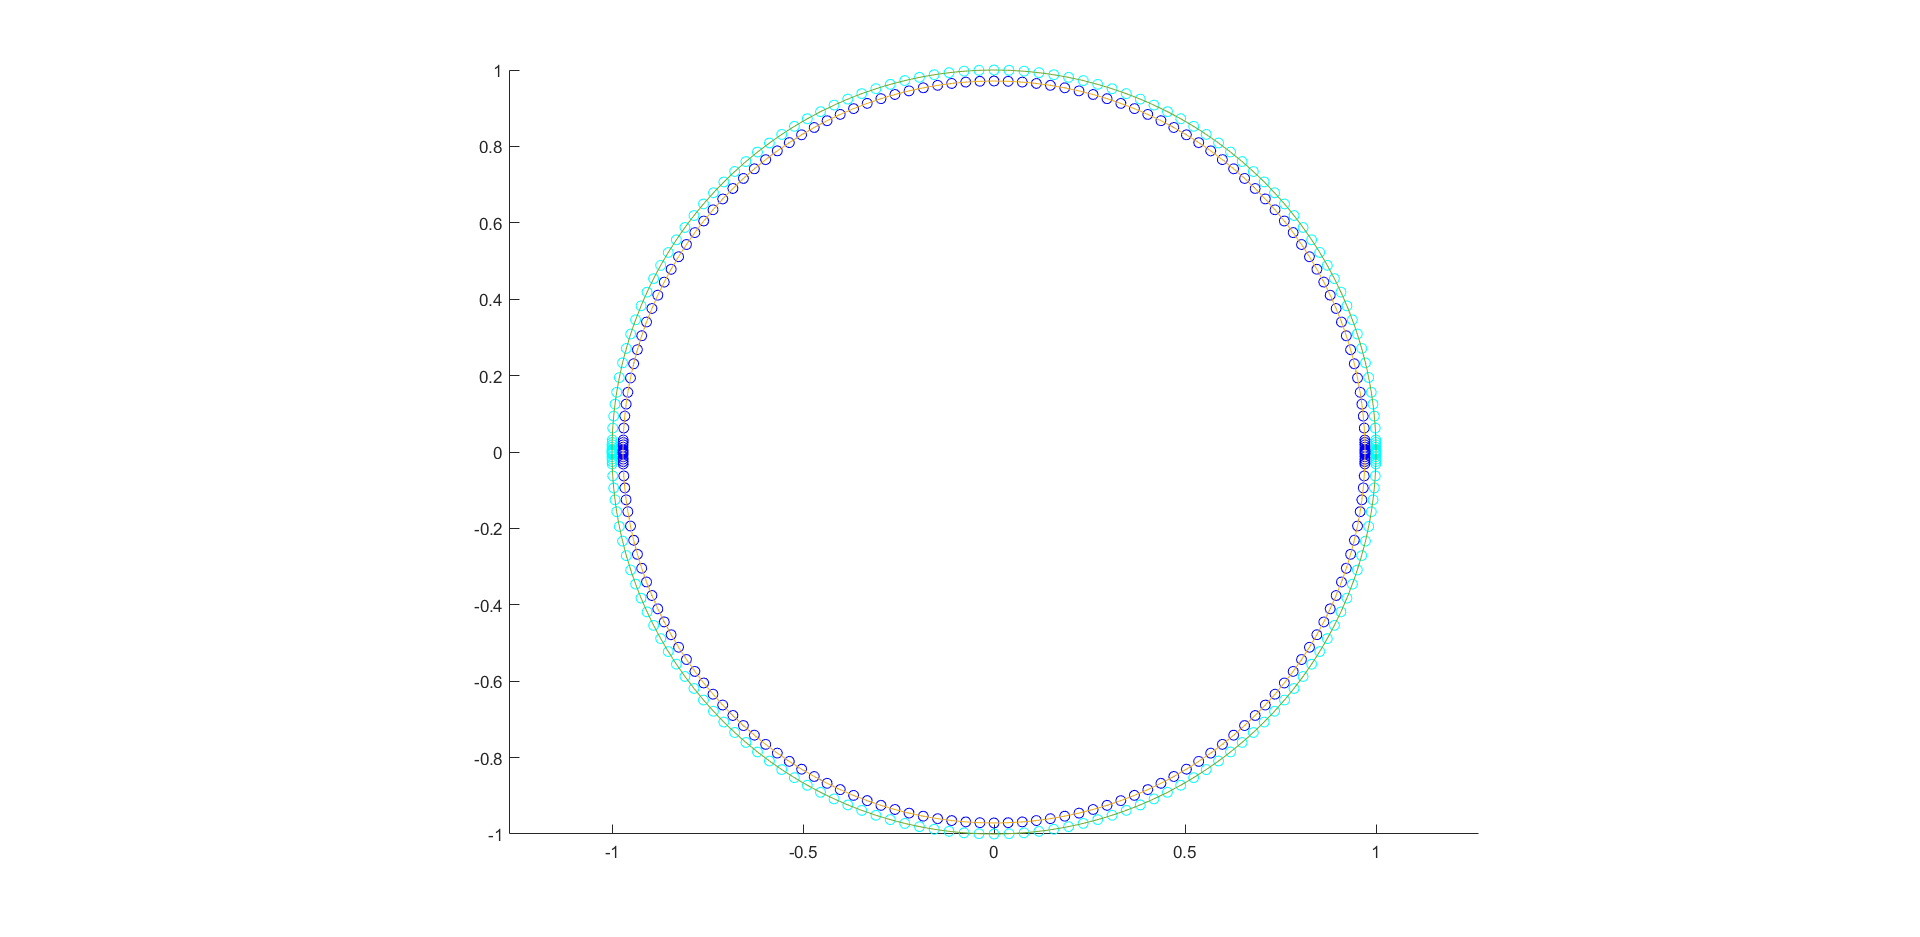
\includegraphics[width=1\textwidth]{fig/Q3-NEW.png}   %以行宽的0.5倍大小显示
	\caption{Result} 
	\label{fig1}  %图片引用标记
\end{figure}


The figure 1 shows the solutions of the BVP by analytic solution and the numerial solution in question 2. To plot the following figure, change the parameter p, then hold on the figure. Then the result is shown in figure 1. The Matlab code can be found at \textbf{solveQ2.m} file. For $p=0$, the analytical solution is green, the numerical solution is cyan. For $p=3$, the numerial solution is blue, the analytical solution is orange.

%--------------------------------------------------
%--------------------------------------------------


%--------------------------------------------------
%--------------------------------------------------

\section*{Question 4} 
Change pressure to p = 3.5, and resolve the BVP. Note that the solution obtained depends
on the initial condition used for Broyden’s Method II. Plot each different solution found.
%--------------------------------------------------
%--------------------------------------------------


\textbf{Solution:} 
The parameter are $c=0.01$, $p=3.5$, $k=100$, then we need to try different sets of parameters to find the three different solutions. Hence, we tried s0 = [2;1;0]; s0 = [-1.28;1.8;0]; s0 = [-0.2;0.6;-1.2]. Then we run the script \textbf{solveQ4.m}:

\begin{lstlisting}
clc;
clear;
%% Q4
global c p;
c = 0.01;
p = 3.5; % Change the value of p here

%% Init
s=[0 0 0 0 0 0 0]; 
s0 = [-0.2;0.6;-1.2];
% circular solution: s0 = [2;1;0];
% buckled solution 1: s0 = [-1.28;1.8;0];
% buckled solution 2: s0 = [-0.2;0.6;-1.2];
sspan = [0 pi/2];
y0 = [pi/2 s(2) 0 0 s(5) 0 s(7)];
yb = [0 0 0 0 0 0 0]; %Value to be Shot
k=100;

%% Solver
% z=F(s0, c, p);

sstar = broyden2(@(s)F(s, c, p), s0, k); 

if (norm(F(sstar, c, p)) < 1e-3)
	disp("sstar found")
	% Plot the Result
	y0 = [pi/2 sstar(1) 0 0 sstar(2) 0 sstar(3)]; %Initial State
	[~,w_sol]=ode45(@(s,y) odefcn(y,c,p),sspan,y0);
	
	axis equal 
	hold on
	plot(w_sol(:,2),w_sol(:,3),'b-o'); %LU (You may change color here)
	plot(-w_sol(:,2),w_sol(:,3),'b-o');%RU
	plot(-w_sol(:,2),-w_sol(:,3),'b-o');%RD
	plot(w_sol(:,2),-w_sol(:,3),'b-o');%LD
else
	disp("Failed")
end
\end{lstlisting}

For different initial state, s0 = [2;1;0]; s0 = [-1.28;1.8;0]; s0 = [-0.2;0.6;-1.2]. The corresponding sstar are $\mathbf{sstar}=\left[\begin{array}{l}
	-0.9665 \\
	-3.3828 \\
	-0.0335
\end{array}\right]
$ (blue), $\mathbf{sstar}=\left[\begin{array}{l}
	-0.5879 \\
	-2.0578 \\
	0.9293
\end{array}\right]
$ (Cyan), $\mathbf{sstar}=\left[\begin{array}{l}
	-1.2317 \\
	-4.3109 \\
	-1.206
\end{array}\right]
$ (Red). Then, we hold on graph and plot 3 different sets of solution as shown in figure 2:

\begin{figure}[htbp]  %[htbp]中的h是浮动的意思
	\centering    %居中
	\centering          %子图居中
	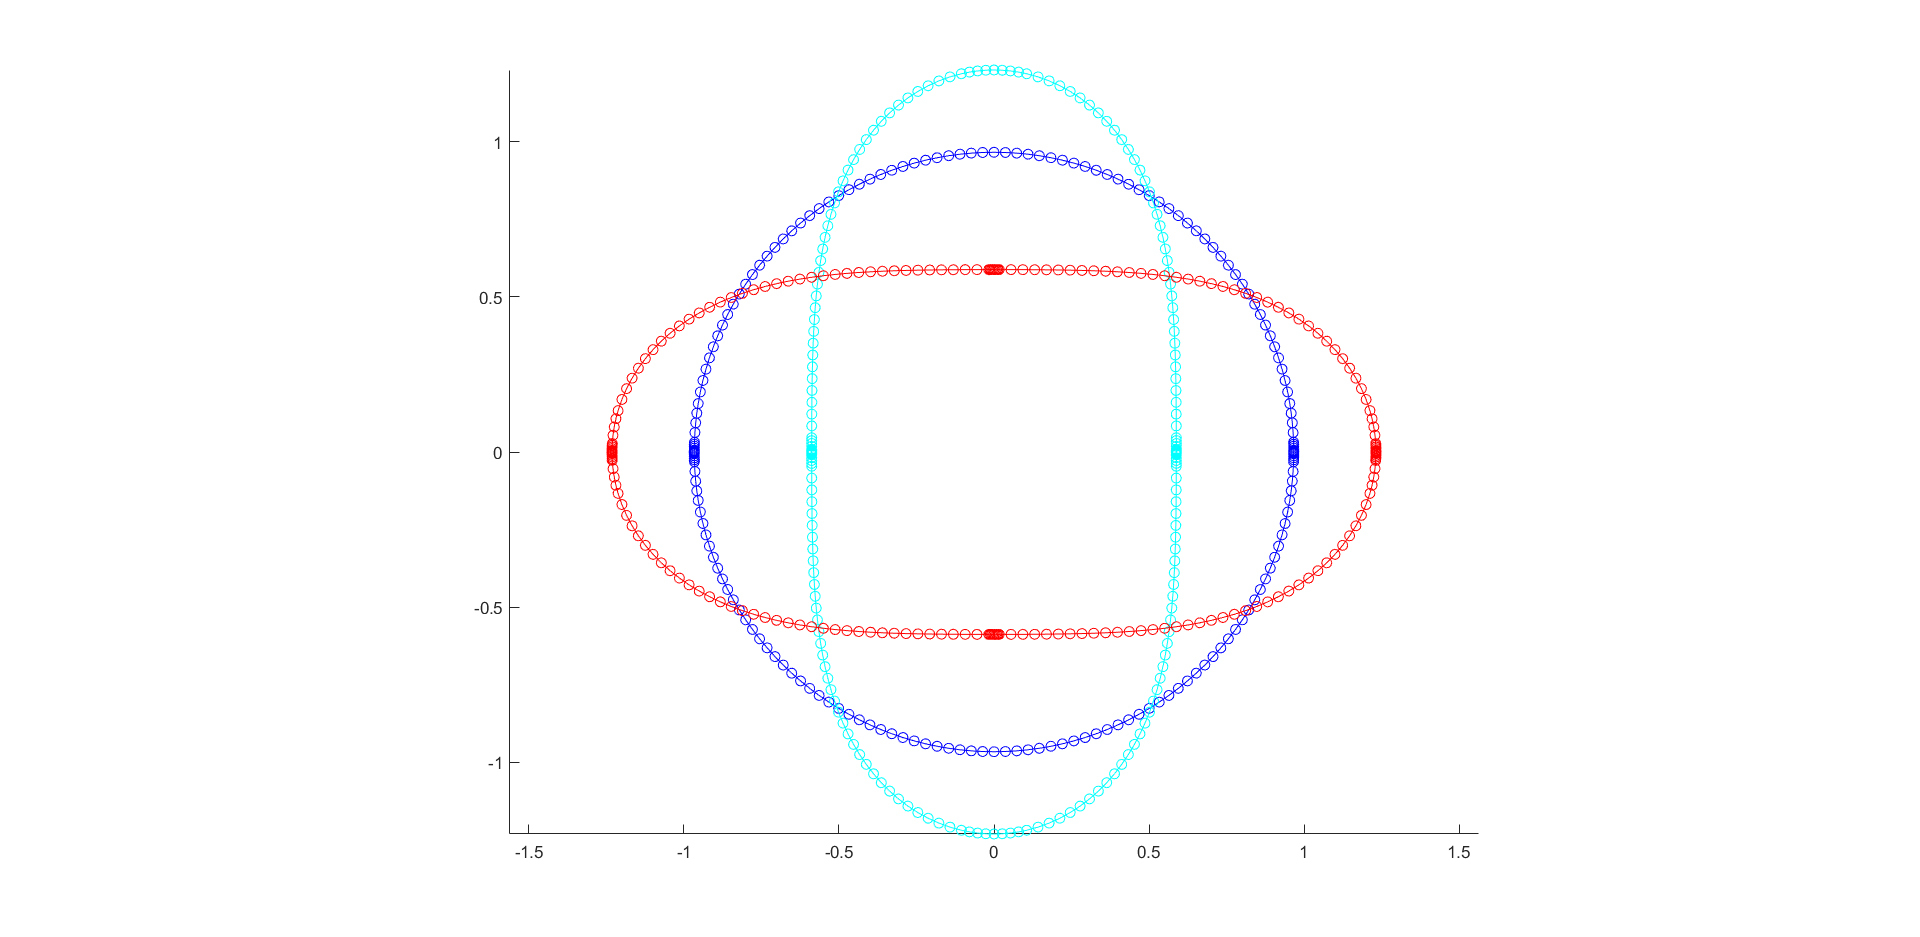
\includegraphics[width=1\textwidth]{fig/Q4-NEW.png}   %以行宽的0.5倍大小显示
	\caption{Result} 
	\label{fig1}  %图片引用标记
\end{figure}


%--------------------------------------------------
%--------------------------------------------------


%--------------------------------------------------
%--------------------------------------------------

\section*{Question 5} 
Find the critical pressure $p_c$ for the compressibility c = 0.01, accurate to two decimal
places. For $p > p_c$, there are three different solutions. For $p < p_c$, there is only one
solution (7.10).
%--------------------------------------------------
%--------------------------------------------------


\textbf{Solution:} 

For applied pressure p below the critical pressure $p_c$, only
solution (7.10) exists. For $p > p_c$, three different solutions of the BVP exist. From the disccusion above, we believe that the $p_c \ \in \ [3,3.5]$. The idea is that if p changes a little, then the solution may change also only a little. So, if we can find a solution at $p_a$, then we can use the solution as a good initial guess at $p_a+ step \ size$., in our case, the step size is $0.01$. 


Then, we run the script many time by changing the s0 and p. Finally, we found the critical pressure is in the smaller inverval $[3.18,3.25]$. 
 


\begin{lstlisting}
clc;
clear;
%% Q4
global c p;
c = 0.01;
p = 3.5; % Change the value of p here

%% Init
s=[0 0 0 0 0 0 0]; 
s0 = [-0.9712;-2.9135;-0.0288];
sspan = [0 pi/2];
y0 = [pi/2 s(2) 0 0 s(5) 0 s(7)];
yb = [0 0 0 0 0 0 0]; %Value to be Shot
k=100;
h=0.001;

%% Solver
% z=F(s0, c, p);
for p = 3: +h:3.5
	sstar = broyden2(@(s)F(s, c, p), s0, k); 
	y0 = [pi/2 sstar(1) 0 0 sstar(2) 0 sstar(3)];
	[~,w_sol]=ode45(@(s,y) odefcn(y,c,p),sspan,y0);
	w_radius = 1 - sqrt(w_sol(end,2)^2 + w_sol(end,3)^2);
	
	sstar2 = broyden2(@(s)F(s, c, p), sstar, k); 
	y0 = [pi/2 sstar2(1) 0 0 sstar2(2) 0 sstar2(3)];
	[~,w_sol2]=ode45(@(s,y) odefcn(y,c,p),sspan,y0);
	w_radius2 = 1 - sqrt(w_sol2(end,2)^2 + w_sol2(end,3)^2);
	
	disp(w_radius);
	disp(w_radius2);
	
	if (abs(w_radius - w_radius2) > 1e-1)
		disp("not continuous", sstar);
		break;
	end
	disp(p); 
end
\end{lstlisting}

%--------------------------------------------------
%--------------------------------------------------

\section*{Question 6} 
Carry out Step 5 for the reduced compressibility c = 0.001. The ring now is more brittle.
Is the change in $p_c$ for the reduced compressibility case consistent with your intuition?
%--------------------------------------------------
%--------------------------------------------------


\textbf{Solution:} 



Sure, the $p_c$ increased with my intuition.


%--------------------------------------------------
%--------------------------------------------------



%--------------------------------------------------
%--------------------------------------------------

\section*{Question 7} 

Carry out Step 5 for increased compressibility c = 0.05.
%--------------------------------------------------
%--------------------------------------------------


\textbf{Solution:} 


The methodology is similar in step 5.







%--------------------------------------------------
%--------------------------------------------------

%--------------------------------------------------
%--------------------------------------------------

\section*{References} 

Huddleston, J.V. \& Sivaselvan, M.V. (2000) Buckling and Postbuckling of Compressible Circular Rings Under Hydrostatic Pressure. AIAA Journal. [Online] 38 (12), 2361–2363. Available from: doi:10.2514/2.909.


\end{document}
